
\chapter{Applying the model}

\section{Non-dimensionalising the equations of motion}
In order to non-dimensionalise the equations of motion (EOMs) we
introduce dimensionless parameters $\vb{x}_i = L\hat{\vb{x}}_i$, $t = T \hat{t}$, $b = B \hat{b}$
and $c = C \hat{c}$, where $L, T, B$ and $C$ are general undetermined scalings for the independent 
and dependent variables, respectively. At the outset, we fix $L = L_0$ the nominal major cell diameter, and
$ T = \frac{1}{\mu^*}$ the reciprocal of specific growth rate for yeast, that is the $\mu^* = \mu(0)$ that appears in
the formula for the total cell count (talk about ideal conditions $\mu^* = 0.4$ hour$^{-1}$)
\begin{equation*}  
    N(t) = N_0 e^{ t \mu(t)}.
\end{equation*}
Substituting in these parameters, we obtain 
\begin{equation*}
    \frac{C}{(1/\mu^*)}\pdv{\hat{c}}{\hat{t}} = \left(\frac{D C}{ L_0^2} \right)\left(\pdv[2]{\hat{c}}{\hat{x}} + \pdv[2]{\hat{c}}{\hat{y}} \right) -
      \left( r C B\right)  \hat{c}\hat{b},
\end{equation*}
which results in 
\begin{equation*}
    \pdv{\hat{c}}{\hat{t}} = \left(\frac{D}{ \mu^* L_0^2} \right)\left(\pdv[2]{\hat{c}}{\hat{x}} + \pdv[2]{\hat{c}}{\hat{y}} \right) -
      \left( \frac{r  B}{\mu^*}\right)  \hat{c}\hat{b}.
\end{equation*}
Call the dimensionless diffusion constant $\lambda_1 = \frac{D}{ \mu^* L_0^2}$ and 
set $\frac{r  B}{\mu^*}=1$ which are free to do since $B$ is unset to begin with. This means 
that the scaling for the biomass density is $B = \frac{\mu^*}{r}$. The reaction diffusion equation 
reduces to 
\begin{equation*}
    \pdv{\hat{c}}{\hat{t}} = \lambda_1 \left(\pdv[2]{\hat{c}}{\hat{x}} + \pdv[2]{\hat{c}}{\hat{y}} \right) -
      \hat{c}\hat{b}.
\end{equation*}
Now, for the EOM for the nodes, we have
\begin{equation*}
    \begin{split}
        \frac{d \vb{x}_i}{dt} &= 
        \frac{K}{ \eta}\sum_{j = 1}^N   \left[ - A_{ij} \left( ||\vb{x}_i - \vb{x}_j|| - L_0\right) \frac{\vb{x}_i - \vb{x}_j}{||\vb{x}_i - \vb{x}_j||} \right]\\
         &+ \frac{F}{ \eta}\sum_{j = 1}^N \left[ H(R - ||\vb{x}_i - \vb{x}_j||) \frac{\vb{x}_i - \vb{x}_j}{||\vb{x}_i - \vb{x}_j||}     \right]\\ 
         &+ \frac{\gamma}{\eta} \nabla c (\vb{x}_i, t).
    \end{split}
\end{equation*}
Substituting the dimensionless parameters, we acquire
\begin{equation*}
    \begin{split}
        \frac{L_0}{(1/\mu^*)}\frac{d \hat{\vb{x}}_i}{d \hat{t}} &= 
        \frac{K L_0}{ \eta}\sum_{j = 1, j \neq i}^N   \left[ - A_{ij}\left( ||\hat{\vb{x}}_i - \hat{\vb{x}}_j|| -  1\right) \frac{\hat{\vb{x}}_i - \hat{\vb{x}}_j}{||\hat{\vb{x}}_i - \hat{\vb{x}}_j||} \right]\\
         &+ \frac{F}{  \eta}\sum_{j = 1, j \neq i}^N \left[H(\hat{R} - ||\hat{\vb{x}}_i - \hat{\vb{x}}_j||) \frac{\hat{\vb{x}}_i - \hat{\vb{x}}_j}{||\hat{\vb{x}}_i - \hat{\vb{x}}_j||}     \right]\\ 
         &+ \frac{\gamma C}{ \eta L_0} \hat{\nabla}  \hat{c} (\hat{\vb{x}}_i, \hat{t}),
    \end{split}
\end{equation*}
which, after rearrging, becomes,
\begin{equation*}
    \begin{split}
        \frac{d \hat{\vb{x}}_i}{d \hat{t}} &= 
        \frac{K}{ \eta \mu^*}\sum_{j = 1, j \neq i}^N   \left[ - A_{ij}\left( ||\hat{\vb{x}}_i - \hat{\vb{x}}_j|| -  1\right) \frac{\hat{\vb{x}}_i - \hat{\vb{x}}_j}{||\hat{\vb{x}}_i - \hat{\vb{x}}_j||} \right]\\
         &+ \frac{F}{  \eta \mu^* L_0}\sum_{j = 1, j \neq i}^N \left[H(\hat{R} - ||\hat{\vb{x}}_i - \hat{\vb{x}}_j||) \frac{\hat{\vb{x}}_i - \hat{\vb{x}}_j}{||\hat{\vb{x}}_i - \hat{\vb{x}}_j||}     \right]\\ 
         &+ \frac{\gamma C}{ \eta \mu^* L_0^2} \hat{\nabla}  \hat{c} (\hat{\vb{x}}_i, \hat{t}).
    \end{split}
\end{equation*}
Only one of the coefficients could be set to unity, but instead we choose $C = c_0 = 1$ to be the initial 
concentration. That leaves us with four additional parameters,
\begin{equation*}
    \lambda_2 = \frac{K}{ \eta \mu^*},
\end{equation*}
\begin{equation*}
    \lambda_3 = \frac{F}{  \eta \mu^* L_0},
\end{equation*}
\begin{equation*}
    \lambda_4 = \frac{R}{L_0},
\end{equation*}
\begin{equation*}
    \lambda_5 = \frac{\gamma c_0}{ \eta \mu^*L_0^2}.
\end{equation*}
 We also think of the biomass
field as being directly equal (in units) to the total signed distance field (rather than just proportial to).
So, we are left with the following EOM for the biomass field,
\begin{equation*}
    B\hat{b} = \begin{cases}
                -  L_0\hat{g}(\hat{x},\hat{y},\hat{t}), & \ \textrm{if} \ \hat{g}(\hat{x},\hat{y},\hat{t}) \leq 0, \\
                    0, &    \ \textrm{otherwise}.
               \end{cases}
\end{equation*}
\begin{equation*}
    \hat{b} = \begin{cases}
                -  \frac{r L_0}{\mu^*}\hat{g}(\hat{x},\hat{y},\hat{t}), & \ \textrm{if} \ \hat{g}(\hat{x},\hat{y},\hat{t}) \leq 0, \\
                    0, &    \ \textrm{otherwise}.
               \end{cases}
\end{equation*}
which leaves us with an additional parameter, $\lambda_6 =\frac{r L_0}{\mu^*}$. The final model parameter is the cell aspect ratio, $\lambda_7$.


\begin{table}[h]
\begin{center}
    \begin{tabular}{ |c|c|c| } 
     \hline
      \textbf{Symbol} & \textbf{Expression} & \textbf{Descriptive name} \\ 
      \hline
     $\lambda_1$ & $\frac{D}{ \mu^* L_0^2}$ & diffusivity \\ 
     $\lambda_2$ & $\frac{K}{ \eta \mu^*}$ & elasticity \\ 
     $\lambda_3$ & $\frac{F}{  \eta \mu^* L_0}$ & respulsivity \\ 
     $\lambda_4$ & $\frac{R}{L_0}$ & respulsion radius \\ 
     $\lambda_5$ & $\frac{\gamma c_0}{ \eta \mu^* L_0^2}$ & mobility \\ 
     $\lambda_6$ & $\frac{r L_0}{\mu^*}$ & metabolic rate \\ 
     $\lambda_7$ & $\frac{\textrm{cell minor axis}}{\textrm{cell major axis}}$ & cell aspect ratio \\ 
     \hline
     
    \end{tabular}
    
\end{center}
\caption{A summary of the dimensionless model parameters}
\end{table}

Dropping the hats on variable symbols, we arive at the final system equations of motion.
\newpage


\begin{equation} \label{eqn:EOMs_PDE}
    \boxed{\pdv{c}{t} = \lambda_1 \left(\pdv[2]{c}{x} + \pdv[2]{c}{y} \right) - bc,
     \ \textrm{for} \ (x,y) \in \Omega \setminus \partial \Omega,}
\end{equation}
\begin{equation} \label{eqn:EOMs_PDE_boundary}
    \boxed{c(x,y,t) = 1, \ \textrm{for} \ (x,y) \in \partial \Omega,}
\end{equation}
\begin{equation} \label{eqn:EOMs_PDE_initial}
    \boxed{c(x,y,0) = 1,}
\end{equation}

\begin{equation} \label{eqn:EOMs_ODEs}
    \boxed{
    \begin{split}
        \frac{d \vb{x}_i}{d t} 
         &= \lambda_2 \sum_{j=1}^{N_{\textrm{nodes}}} \left[ A_{ij}\left( 1- ||\vb{x}_i - \vb{x}_j|| \right) \frac{\vb{x}_i - \vb{x}_j}{||\vb{x}_i - \vb{x}_j||} \right]\\
         &+ \lambda_3 \sum_{j=1}^{N_{\textrm{nodes}}} \left[H(\lambda_4 - ||\vb{x}_i - \vb{x}_j||) \frac{\vb{x}_i - \vb{x}_j}{||\vb{x}_i - \vb{x}_j||}     \right]\\ 
         &+ \lambda_5 \nabla c (\vb{x}_i, t), \ \textrm{for} \ i \in \{ 1, ...,N_{\textrm{nodes}} \},  
    \end{split}}
\end{equation}
\begin{equation} \label{eqn:EOMs_ODEs_initial}
    \boxed{\vb{x}_1(0) = (-0.5, 0), \ \vb{x}_2(0) = (0.5, 0), }
\end{equation}
\begin{equation} \label{eqn:EOMs_N_nodes}
    \boxed{N_{\textrm{nodes}} = N_0 e^{t \mu(t)}, \textrm{where} \ N_0 = 1, }
\end{equation}
\begin{equation} \label{eqn:EOMs_growth_rate}
    \boxed{\mu(t) = \frac{1}{N_{\textrm{nodes}}}\sum_{j=1}^{N_{\textrm{nodes}}} c(\vb{x}_j, t), } 
\end{equation}
\begin{equation}
    \boxed{
    b(x,y,t) = 
    \begin{cases}
        -\lambda_6 g(x,y,t), & \ \textrm{if} \ g(x,y,t) \leq 0, \\
            0, &    \ \textrm{otherwise},
    \end{cases}
    }
\end{equation}
\begin{equation}
    \boxed{
    g(x,y,t) = \min_{k \in \{  1, ..., N_{\textrm{cells}}\}} f_k (x,y,t),
    }
\end{equation}
\begin{equation}
    \boxed{
    \begin{split}
    f_k(x,y,t) &= \left[\frac{ (x-x_{c,k}(t))\cos{\theta_k} + (y-y_{c,k}(t)) \sin{\theta_k}}{a_k(t)} \right]^2 \\ 
               &+ \left[ \frac{-(x-x_{c,k}(t))\sin{\theta_k} +(y-y_{c,k}(t)) \cos{\theta_k}}{b_k(t)} \right]^2 - 1,
    \end{split}
    }
\end{equation}
\begin{equation} \label{eqn:EOMs_growth_rate}
    \boxed{a_k(t) = ||\vb{x}_{j_1} - \vb{x}_{j_2}||, \ 
    \textrm{where cell} \ k \ \textrm{is comprised of nodes} \ j_1, j_2,} 
\end{equation}
\begin{equation} \label{eqn:EOMs_growth_rate}
    \boxed{b_k(t) = \lambda_7 a_k(t), }
\end{equation}
\begin{equation} \label{eqn:EOMs_growth_rate}
    \boxed{\theta_k(t) = \atan (y_{j_1} - y_{j_2},x_{j_1} - x_{j_2} ), }
\end{equation}
\begin{equation} \label{eqn:EOMs_ODEs_initial}
    \boxed{ \vb{x}_{c,k}(t) = \frac{1}{2} \left(\vb{x}_{j_1}(t) + \vb{x}_{j_2}(t)\right). }
\end{equation}

Note that $i$ and $j$ index over node numbers, $k$ over cells, and $j_1$ and $j_2$ denote the nodes
that comprise cell $k$. Finally the petri-dish domain is given by 

\begin{equation}
    \boxed{\Omega = \left[-\frac{1}{2}L_{\textrm{petri-dish}},\frac{1}{2}L_{\textrm{petri-dish}} \right] \times
             \left[-\frac{1}{2}L_{\textrm{petri-dish}},\frac{1}{2}L_{\textrm{petri-dish}} \right] \subset \mathbb{R}^2.}
\end{equation}

\section{From qualitative to quantitative}
The model developed thus far is a numerical framwork for simulating growing cell colonies.
There is an element of randomness in the model: when two nodes are dislodged from the 
same point there is initially no preferred direction to move in so one must be chosen randomly
before other forces can take effect. For this reason, every seperate run of the model 
starting with identical initial conditions will look very different after time has passed. 
It is expected however that some ``averaged''
quantity will stabilise so long as the model is simulated over a fairly large number of runs.
Seperate runs of the model belong to a set called an ensemble.
We will start with a relatively straightforward metric, the number of cells at time
$T = 500$ steps.

\newpage

\begin{figure}[!htb] %Change this to [p] maybe ?
    \centering
    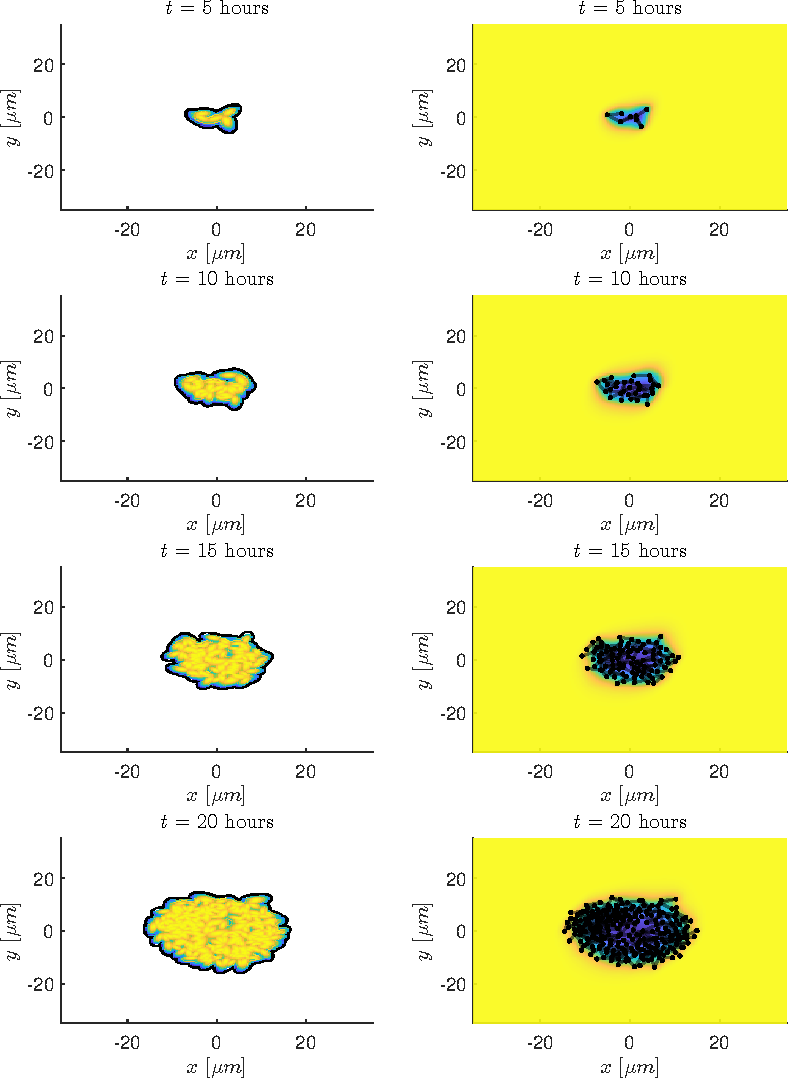
\includegraphics[width= 1\textwidth]{
        chapter2/figures/t_all_L1_0o10_L2_1o00_L3_1o00_L4_0o50_L5_1o00_L6_0o30_L7_0o50.pdf}
    \caption{A cell colony with parameter values given by
             $\lambda_1 = 0.1$,  
             $\lambda_2 = 1.0$, 
             $\lambda_3 = 1.0$, 
             $\lambda_4 = 0.5$, 
             $\lambda_5 = 1.0$, 
             $\lambda_6 = 0.3$, 
             $\lambda_7 = 0.5$. 
             On the left we have the biomass field, the nutrient field is on the right.}
    \label{fig: sdsd}
\end{figure}


\newpage


\begin{figure}[!htb] %Change this to [p] maybe ?
    \centering
    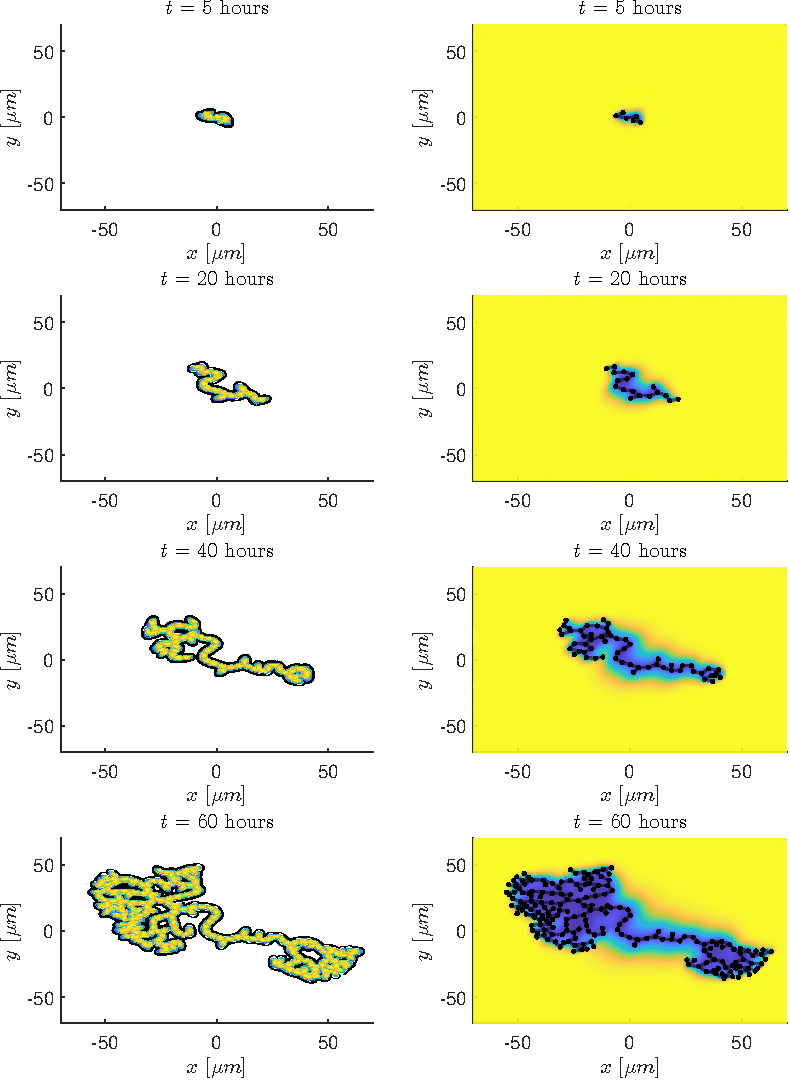
\includegraphics[width= 1\textwidth]{
        chapter2/figures/t_all_L1_0o10_L2_1o00_L3_1o00_L4_0o50_L5_1o00_L6_2o00_L7_0o50.pdf}
    \caption{A cell colony with parameter values given by
             $\lambda_1 = 0.1$,  
             $\lambda_2 = 1.0$, 
             $\lambda_3 = 1.0$, 
             $\lambda_4 = 0.5$, 
             $\lambda_5 = 1.0$, 
             $\lambda_6 = 2.0$, 
             $\lambda_7 = 0.5$. 
             Biomass on left and nutrient field on the right.}
    \label{fig: sdsd}
\end{figure}

\newpage

\begin{figure}[!htb] %Change this to [p] maybe ?
    \centering
    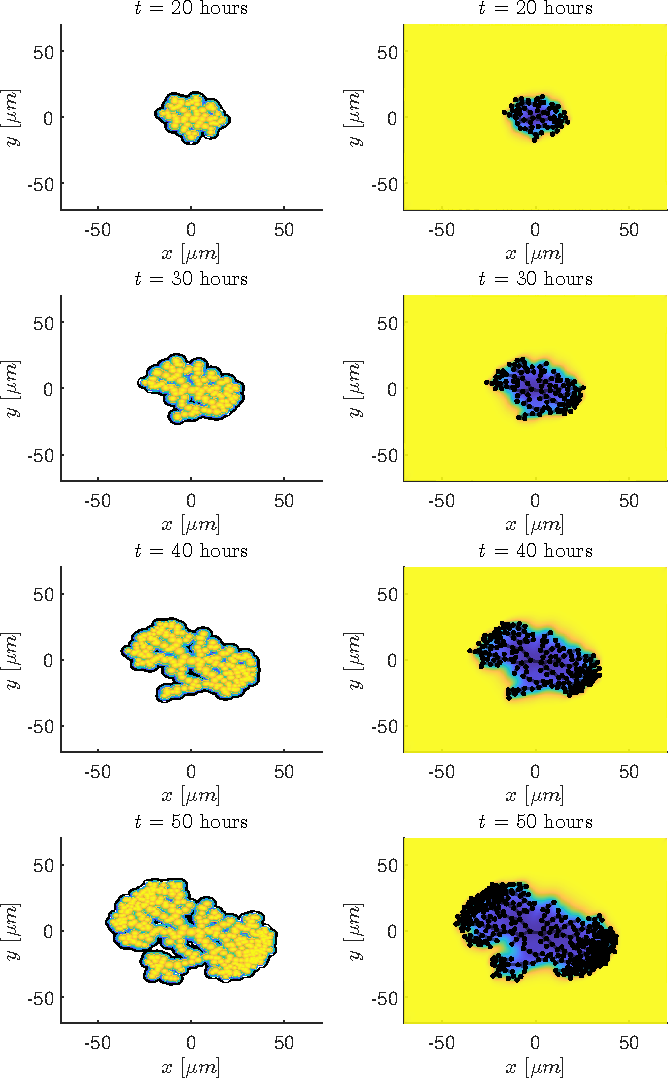
\includegraphics[width= 1\textwidth]{
        chapter2/figures/t_all__L1_0o10_L2_1o00_L3_1o00_L4_0o50_L5_1o00_L6_0o50_L7_1o00.pdf}
    \caption{A cell colony with parameter values given by
             $\lambda_1 = 0.1$,  
             $\lambda_2 = 1.0$, 
             $\lambda_3 = 1.0$, 
             $\lambda_4 = 0.5$, 
             $\lambda_5 = 1.0$, 
             $\lambda_6 = 0.5$, 
             $\lambda_7 = 1.0$. 
             Biomass on left and nutrient field on the right.}
    \label{fig: sdsd}
\end{figure}


\begin{figure}[h] %Change this to [p] maybe ?
    \centering
    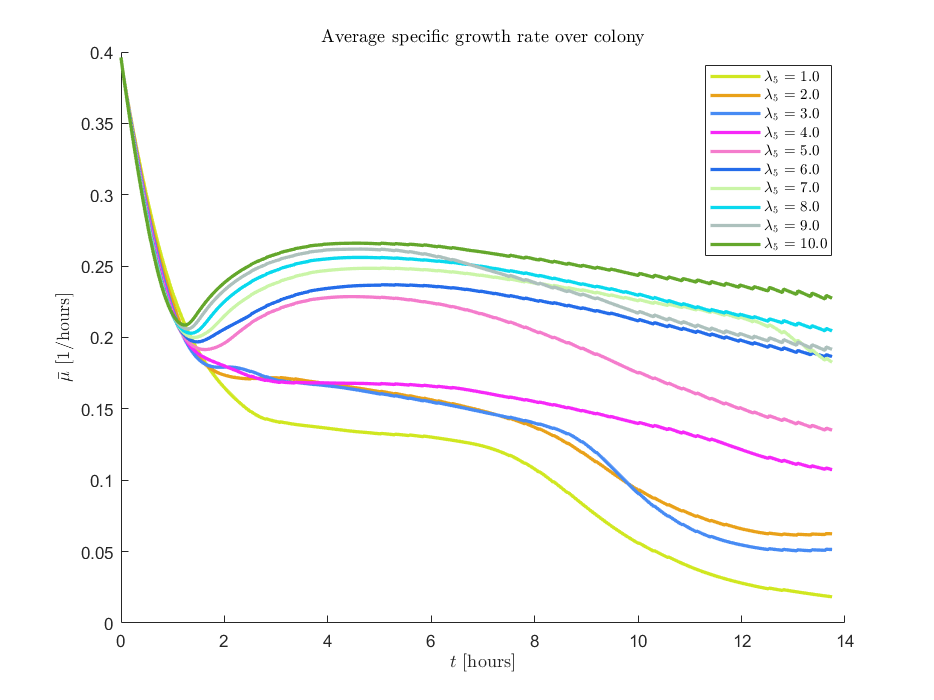
\includegraphics[width= 1\textwidth]{
        chapter2/figures/SpecificGrowthRatePlot.png}
    \caption{The colony average specific growth rate for different values of $\lambda_5$
                is measured and plotted over time for ensemble size $1$. The rest of the parameters 
                took the values:
                $\lambda_1 = 0.1$,  
                $\lambda_2 = 1.0$, 
                $\lambda_3 = 1.0$, 
                $\lambda_4 = 1.0$, 
                $\lambda_5$ (variable), 
                $\lambda_6 = 0.5$, 
                $\lambda_7 = 0.7$.
                Remarkably, when $\lambda_5 \geq 5.0$ there is an interesting dynamic that 
                occurs based on the compettition between nutrient consumption rate ($\lambda_6$)
                and the mobility ($\lambda_5$). For small values of mobility,
                the cells are not able to move enough into areas where the nutrient has not 
                decayed.}
    \label{fig:ColonySimulationNutrientFieldN210}
    \end{figure}
    \filbreak

\begin{figure}[h]
    \centering
    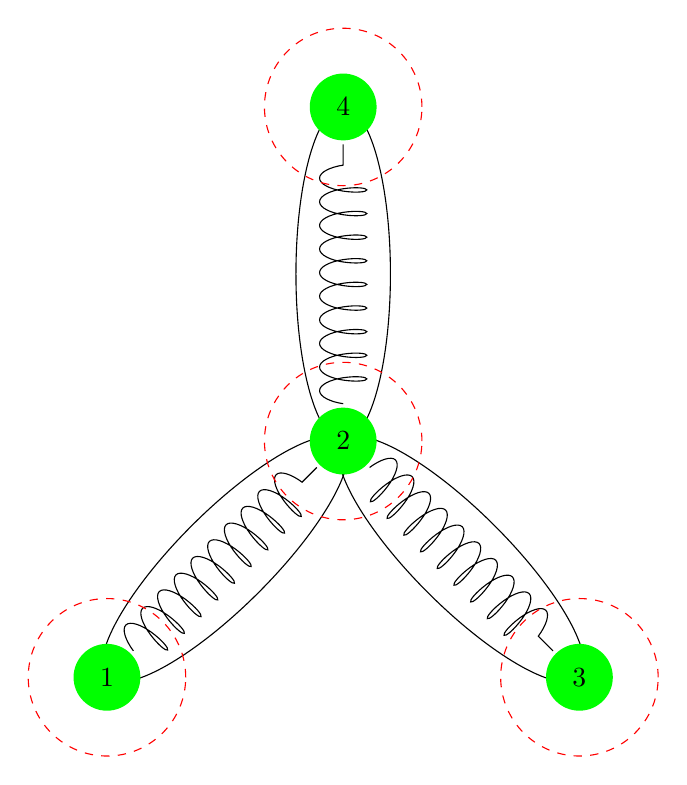
\begin{tikzpicture}
        \draw[rotate=45] (-0.5*4.243cm,0) ellipse (0.5*4.243cm and 0.6cm);
        \draw[rotate=-45] (0.5* 4.243,0) ellipse (0.5*4.243cm and 0.6cm);
        \draw[rotate=0] (0.0,0.5* 4.243)  ellipse (0.6cm and 0.5*4.243cm);
        
        \node[circle,fill=green, line width=1mm,inner sep=2.0mm] (a) at (-3,-3)  {1};
        \node[circle,fill=green, line width=1mm,inner sep=2.0mm] (b) at (0,  0)  {2};
        \node[circle,fill=green, line width=1mm,inner sep=2.0mm] (c) at (3, -3)  {3};
        \node[circle,fill=green, line width=1mm,inner sep=2.0mm] (d) at (0,4.243){4};
        \draw[decoration={aspect=0.3, segment length=3mm, amplitude=3mm,coil},decorate] (a) -- (b);
        \draw[decoration={aspect=0.3, segment length=3mm, amplitude=3mm,coil},decorate] (b) -- (c);  
        \draw[decoration={aspect=0.3, segment length=3mm, amplitude=3mm,coil},decorate] (b) -- (d); 

        \draw[dashed, color=red]   (a)  ellipse (1.0cm and 1.0cm);
        \draw[dashed, color=red]   (b)  ellipse (1.0cm and 1.0cm);
        \draw[dashed, color=red]   (c)  ellipse (1.0cm and 1.0cm);
        \draw[dashed, color=red]   (d)  ellipse (1.0cm and 1.0cm);
    \end{tikzpicture}
    \caption{A diagram of three elliptical cells with internal springs to represent biomass 
             elasticity ($\lambda_2 = \frac{K}{\eta \mu}$). The nodes are positioned at the ends of the major dimension
             of each ellipse and there are two nodes per cell. The force acting on 
             node $2$ for instance would be due to the forces from nodes $1$, $3$ and $4$.
             The dashed red circles represent the activation radius ($ \lambda_4 = R/L_0$) 
             of the contact force between the nodes.}
\end{figure}


\begin{figure}[h]
    \centering
    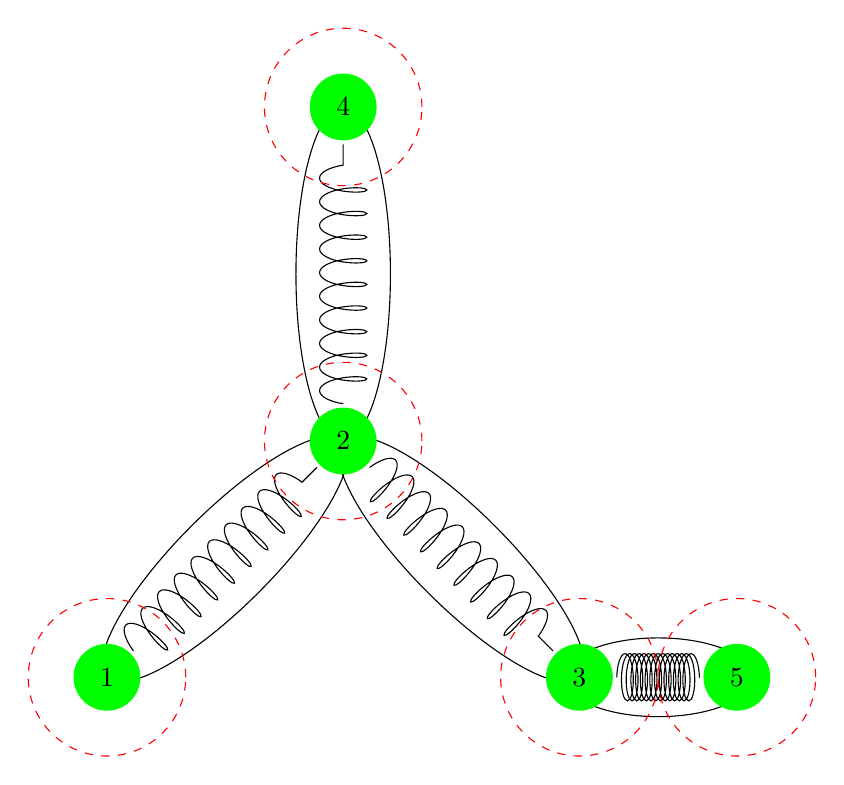
\begin{tikzpicture}
        \draw[rotate=45] (-0.5*4.243cm,0) ellipse (0.5*4.243cm and 0.6cm);
        \draw[rotate=-45] (0.5* 4.243,0) ellipse (0.5*4.243cm and 0.6cm);
        \draw[rotate=0] (0.0,0.5* 4.243)  ellipse (0.6cm and 0.5*4.243cm);
        \draw[rotate=0] (4.0,-3.0)  ellipse (1.2cm and 0.5cm);

        \node[circle,fill=green, line width=1mm,inner sep=2.0mm] (a) at (-3,-3)  {1};
        \node[circle,fill=green, line width=1mm,inner sep=2.0mm] (b) at (0,  0)  {2};
        \node[circle,fill=green, line width=1mm,inner sep=2.0mm] (c) at (3, -3)  {3};
        \node[circle,fill=green, line width=1mm,inner sep=2.0mm] (d) at (0,4.243){4};
        \node[circle,fill=green, line width=1mm,inner sep=2.0mm] (e) at (5,-3){5};
        \draw[decoration={aspect=0.3, segment length=3mm, amplitude=3mm,coil},decorate] (a) -- (b);
        \draw[decoration={aspect=0.3, segment length=3mm, amplitude=3mm,coil},decorate] (b) -- (c);  
        \draw[decoration={aspect=0.3, segment length=3mm, amplitude=3mm,coil},decorate] (b) -- (d); 
        \draw[decoration={aspect=0.3, segment length=0.6mm, amplitude=3mm,coil},decorate] (c) -- (e); 

        \draw[dashed, color=red]   (a)  ellipse (1.0cm and 1.0cm);
        \draw[dashed, color=red]   (b)  ellipse (1.0cm and 1.0cm);
        \draw[dashed, color=red]   (c)  ellipse (1.0cm and 1.0cm);
        \draw[dashed, color=red]   (d)  ellipse (1.0cm and 1.0cm);
        \draw[dashed, color=red]   (e)  ellipse (1.0cm and 1.0cm);
    \end{tikzpicture}
    \caption{A mitosis event occurs via the addition of new nodes connected to old nodes.
             The nodes are added very close (distance $\delta \ll 1$) by the original nodes (exaggerated here)
             so that the spring force can be defined. After this point, 
             the initially compressed cell ``grows" outwards to achieve its nominal length, under 
             the influence of elasticity, contact and chemotactic forces.}
\end{figure}


\section{Updating the nutrient field in time}
In order to advance the nutrient field in time, an efficient and stable numerical solver
was required. Because of the fact that the nutrient field $\hat{c}(\hat{x},\hat{y},\hat{t})$ is coupled 
to the biomass field which is dependent on a discrete network that changes in connectivity and 
node count, it was necessary to implement the method in-house, as opposed to 
using a pre-existing MATLAB boundary value solver for instance. The Crank-Nicolson method (\cite{crank1947practical}) was 
chosen for the practical reason that it led to faster simulations overall since a larger
time step could be used as opposed to the explicit forward in time central in space (FTCS) scheme. This 
is a direct consequence of the fact that the (implicit) Crank-Nicholson scheme is unconditionally numerically 
stable. Let us begin by verifying this fact using the what is
known as Von Neumann stability analysis (\cite{charney1950numerical}).
\\
\\

From this point we drop the hat on the PDE variables. Firstly, we 
define the nutrient field as $c_{j,k}^{n} = c(x_j, y_k, t_n)$ and similarly for $b_{j,k}^{n}$,
the biomass. The values  $c_{i,j}^{n}$ precisely satisfy the discretised equations which follow.
Let  $\bar{c}_{j,k}^{n}$ be the solution achieved with finite precison arithmetic 
operations which does not necessarily satisfy the equations, up to some error term,
\begin{equation*}
    \epsilon_{j,k}^n = \bar{c}_{j,k}^{n} - c_{j,k}^{n}.
\end{equation*}
Carrying out the Crank-Nicolson discretisation with the values $c_{j,k}^{n}$, we derive
\begin{equation*}
    \frac{c_{j,k}^{n+1} - c_{j,k}^{n}}{\Delta t} =
    \frac{\lambda_1}{2} \left( \nabla^2 c_{j,k}^{n+1} + \nabla^2 c_{j,k}^{n} \right) -
     \frac{1}{2} b_{j,k}^{n} (c_{j,k}^{n+1} + c_{j,k}^{n}),
\end{equation*}


\begin{equation*}
    \begin{split}
        \frac{c_{j,k}^{n+1} - c_{j,k}^{n}}{\Delta t} &=
        \frac{\lambda_1}{2}  \left( \frac{c_{j+1,k}^{n+1} - 2 c_{j,k}^{n+1} + c_{j-1,k}^{n+1} }{h^2} + 
                                    \frac{c_{j,k+1}^{n+1} - 2 c_{j,k}^{n+1} + c_{j,k-1}^{n+1} }{h^2} \right)  \\
                                   & +\frac{\lambda_1}{2} \left( \frac{c_{j+1,k}^{n} - 2 c_{j,k}^{n} + c_{j-1,k}^{n} }{h^2} + 
                                    \frac{c_{j,k+1}^{n} - 2 c_{j,k}^{n} + c_{j,k-1}^{n} }{h^2} \right) \\
                                   &-\frac{1}{2} b_{j,k}^{n} (c_{j,k}^{n+1} + c_{j,k}^{n}).
    \end{split}
\end{equation*}
To evaluate the numerical stability, we introduce a constant $\alpha = \frac{ \lambda_1 \Delta t }{h^2}$.
With this constant in place, we continue with
\begin{equation*}
    \begin{split}
        c_{j,k}^{n+1} - c_{j,k}^{n} &=
       \frac{\alpha}{2}  \left( c_{j+1,k}^{n+1} + c_{j-1,k}^{n+1} + 
                       c_{i,j+1}^{n+1} + c_{j,k-1}^{n+1}  \right) - 2 \alpha c_{j,k}^{n+1}  \\
                                   & +\frac{\alpha}{2} \left( c_{j+1,k}^{n}+ c_{j-1,k}^{n} + 
                                    c_{j,k+1}^{n} + c_{j,k-1}^{n}  \right) - 2 \alpha c_{j,k}^{n} \\
                                   &-\frac{\Delta t}{2} b_{j,k}^{n} (c_{j,k}^{n+1} + c_{j,k}^{n}).
    \end{split}
\end{equation*}
Since the discretised equations are linear in $c_{j,k}^{n}$ (taking $b_{j,k}^{n}$ to be slowly varying)
and since $\bar{c}_{j,k}^n$ also form a solution, the $\epsilon_{j,k}^n$ are also 
a solution.
\begin{equation*}
    \begin{split}
        \epsilon_{j,k}^{n+1} - \epsilon_{j,k}^{n} &=
       \frac{\alpha}{2}  \left( \epsilon_{j+1,k}^{n+1} + \epsilon_{j-1,k}^{n+1} + 
                                \epsilon_{j,k+1}^{n+1} + \epsilon_{j,k-1}^{n+1}  \right) - 2 \alpha \epsilon_{j,k}^{n+1}  \\
                                   & +\frac{\alpha}{2} \left( \epsilon_{j+1,k}^{n}+ \epsilon_{j-1,k}^{n} + 
                                   \epsilon_{j,k+1}^{n} + \epsilon_{j,k-1}^{n}  \right) - 2 \alpha \epsilon_{j,k}^{n} \\
                                   &-\frac{\Delta t}{2} b_{j,k}^{n} (\epsilon_{j,k}^{n+1} + \epsilon_{j,k}^{n}).
    \end{split}
\end{equation*}
We subsitute in an ansatz for the error term which is standard in Von Neumann stability analysis, namely
\begin{equation*}
    \epsilon_{j,k}^n = \xi^n e^{i \nu_x j h} e^{i \nu_y k h},
\end{equation*}
where $\nu_x$ and $\nu_y$ are wavenumbers and $h$ is the spatial step. Note that $i = \sqrt{-1}$. In order for the numerical
method to be stable, we require that $|\xi| \leq 1$ for all values of the wavenumbers $\nu_x, \nu_y$.
Substituting this expression into the discretised equation for the error, we get,
\begin{equation*}
    \begin{split}
        \xi^{n+1} e^{i \nu_x j h} e^{i \nu_y k h} - \xi^{n} e^{i \nu_x j h} e^{i \nu_y k h} &=
       \frac{\alpha}{2}  \left( \xi^{n+1} e^{i \nu_x (j+1) h} e^{i \nu_y k h} + \xi^{n+1} e^{i \nu_x (j-1) h} e^{i \nu_y k h} \right) \\
       &+ \frac{\alpha}{2}\left( \xi^{n+1} e^{i \nu_x j h} e^{i \nu_y (k+1) h} + \xi^{n+1} e^{i \nu_x j h} e^{i \nu_y (k-1) h}  \right) \\
       &-2 \alpha\xi^{n+1} e^{i \nu_x j h} e^{i \nu_y k h}  \\
       &+\frac{\alpha}{2} \left( \xi^{n} e^{i \nu_x (j+1) h} e^{i \nu_y k h}+ \xi^{n} e^{i \nu_x (j-1) h} e^{i \nu_y k h}\right) \\
       &+ \frac{\alpha}{2}\left(\xi^{n} e^{i \nu_x j h} e^{i \nu_y (k+1) h} + \xi^{n} e^{i \nu_x j h} e^{i \nu_y (k-1) h}  \right) \\
       &-2 \alpha \xi^{n} e^{i \nu_x j h} e^{i \nu_y k h}\\
       &-\frac{\Delta t}{2} b_{j,k}^{n} (\xi^{n+1} e^{i \nu_x j h} e^{i \nu_y k h} + \xi^{n} e^{i \nu_x j h} e^{i \nu_y k h}).
    \end{split}
\end{equation*}
Dividing through by $\xi^{n} e^{i \nu_x j h} e^{i \nu_y k h}$, we attain,
\begin{equation*}
    \begin{split}
        \xi - 1 &=
       \frac{\alpha}{2}  \left( \xi e^{i \nu_x h}+ \xi e^{-i \nu_x h} \right) 
       + \frac{\alpha}{2}\left( \xi  e^{i \nu_y h} + \xi  e^{-i \nu_y h}  \right) 
       -2 \xi \alpha  \\
       &+\frac{\alpha}{2} \left(  e^{i \nu_x  h}+  e^{-i \nu_x h}\right)
       + \frac{\alpha}{2}\left(   e^{i \nu_y h} +   e^{-i \nu_y  h}  \right) 
       -2 \alpha
       -\frac{\Delta t}{2} b_{j,k}^{n} (\xi + 1).
    \end{split}
\end{equation*}
Using the fact that $ \frac{e^{i \nu_x h}+  e^{-i \nu_x h}}{2} = \cos(\nu_x h)$ and similarly for
the other terms, we have,
\begin{equation*}
    \begin{split}
        \xi - 1 &=
         \alpha \xi \cos(\nu_x h) 
       + \alpha \xi \cos(\nu_y h) 
       -2 \alpha \xi   \\
       &+\alpha \cos(\nu_x h) 
       + \alpha \cos(\nu_y h) 
       -2 \alpha
       -\frac{\Delta t}{2} b_{j,k}^{n} (\xi + 1).
    \end{split}
\end{equation*}
Finally, solving for $\xi$, and taking its absolute value we have,
\begin{equation*}
    |\xi| = \left| \frac{1 + \alpha \left[ \cos(\nu_x h) + \cos(\nu_y h) \right] - 2 \alpha -\frac{1}{2} \Delta t b_{j,k}^{n} }
                        {1 -\alpha \left[ \cos(\nu_x h) + \cos(\nu_y h) \right]  + 2 \alpha +\frac{1}{2} \Delta t b_{j,k}^{n}} \right|.
\end{equation*}
In order to complete the analysis, consider when biomass is $b_{j,k}^{n} = 0$. We have the simplified
equation,
\begin{equation*}
    |\xi| = \left| \frac{1 -\alpha(2 - \left[ \cos(\nu_x h) + \cos(\nu_y h) \right]) }
                        {1 +\alpha(2 - \left[ \cos(\nu_x h) + \cos(\nu_y h)\right])} \right|,
\end{equation*}
Which has a numerator less than or equal to $1$ because $\alpha > 0$ and 
$0 \leq 2 - \left[ \cos(\nu_x h) + \cos(\nu_y h) \right] \leq 4$. The denominator is 
always greater than or equal to $1$, which is enough to prove that
the Crank-Nicolson scheme for the standard heat equation is numerically stable.
\\
\\
Whether this generalises to non-zero $b_{j,k}^{n}$ is determined by numerical experiments, and 
indeed for $\alpha = \frac{\lambda_1 \Delta t}{h^2} = \frac{(0.1) (0.01)}{(0.1)^2} = 0.1$, the scheme 
was not found to be unstable. However, for higher values of $\alpha$ it was possible to see spurious 
oscillations in the solution field for $c$ which obviously suggests some form of instability.

\section{ Fast computational software in MATLAB }
The software developed for the computational modelling is recquired
to be fast, accurate and easy to understand.


\begin{figure}
    \centering

\begin{tikzpicture}[every text node part/.style={align=center}, 
                    node distance=2cm]
    \node (start) [startstop] {\codeword{Master.m}};
    \node (in1) [io, below of=start] { Model parameters: $\lambda_1, ... , \lambda_7$ \\
                                       Numerical parameters: $h$, $\Delta t$ \\
                                       Run parameters: \codeword{ensembleSize}, \codeword{sampleTimes}};
    \node (pro1) [process, below of=in1] {\codeword{runSimulation.m}};
    \node (pro2) [process, below of=pro1] {\codeword{ellipse.m}};
    \node (pro3) [process, below of=pro2] {\codeword{updateFood.m}};
    \node (dec1) [decision, below of=pro3, yshift=-1.5cm] {Mitosis Condition};
    \node (pro4) [process, below of=dec1, yshift=-1.5cm] {\codeword{addCell.m}};
    \node (proNothing) [process, left of=pro4, xshift=-1.5cm] {Proceed};
    \node (pro5) [process, below of=pro4] {\codeword{updateNodes.m}};
    %\node (pro5) [process, right of=dec1, xshift=2cm] {Process 2b};
    \node (out1) [io, below of=pro5] {Run Statistics at \codeword{sampleTimes}: \\
                                      \codeword{compactness},
                                      \codeword{averageRadius},
                                      \codeword{cellCount},
                                      $\bar{\mu}$};
    \node (stop) [startstop, below of=out1] {Plot ensemble averaged results};
    \node (for) [process, left of=pro3, xshift=-3.5cm] {Loop over ensemble};
    \node (forTime) [process, right of=pro3,  xshift=3.0cm] {Loop over time};

    \draw [arrow] (start) -- (in1);
    \draw [arrow] (in1) -- (pro1);
    \draw [arrow] (pro1) -- (pro2);
    \draw [arrow] (pro2) -- (pro3);
    \draw [arrow] (pro3) -- (dec1);
    \draw [arrow] (dec1) -| node[anchor=south]{else} (proNothing);
    \draw [arrow] (proNothing) |- node[anchor=south]{} (pro5);
    \draw [arrow] (dec1) -- node[anchor=east]{if}(pro4);
    \draw [arrow] (pro4) -- (pro5);
    \draw [arrow] (pro5) -- (out1);
    \draw [arrow] (out1) -- (stop);
    \draw [arrow] (in1) -| node[anchor=south]{} (for);
    \draw [arrow] (for)  |- node[anchor=south]{} (out1);
    \draw [arrow] (pro1)  -| node[anchor=south]{} (forTime);
    \draw [arrow] (forTime)  |- node[anchor=south]{} (pro5);
    
    %\draw [arrow] (pro2a) -- (out1);
    %\draw [arrow] (out1) -- (stop);

    


\end{tikzpicture}

\caption{A flow chart of \textbf{CellColonySimulator} software package in MATLAB. }

\end{figure}



\begin{figure}
    \centering
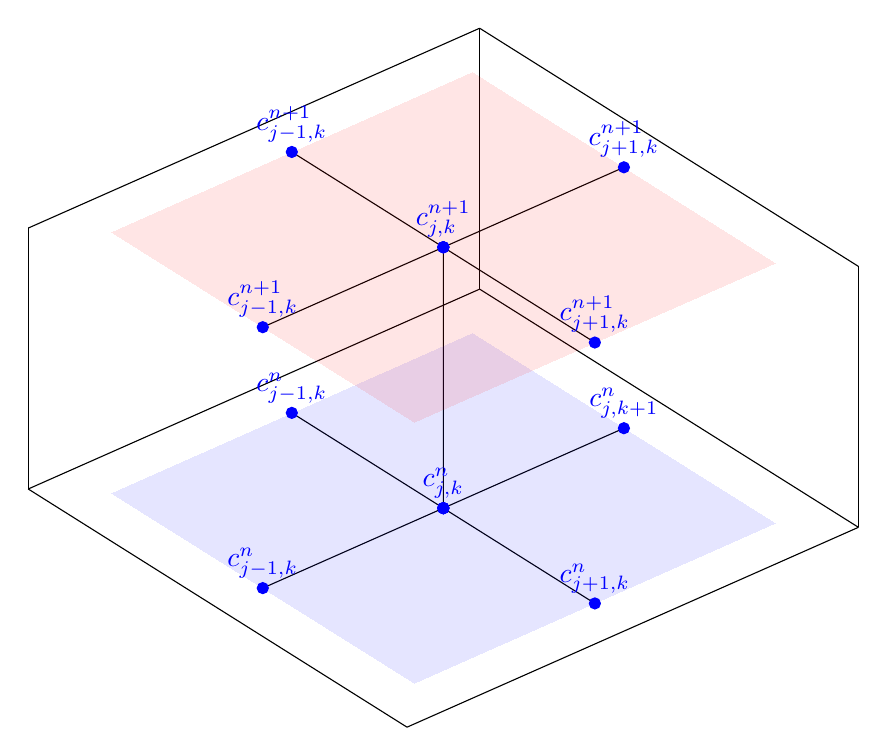
\begin{tikzpicture}
    \pgfplotsset{every tick label/.append style={font=\scriptsize}}
 
    \begin{axis}[view = {50}{50},
        width=\textwidth,
        xmax = 10,
        xmin = -10,
        ymax = 10, 
        ymin = -10, 
        zmax = 10, 
        zmin = 0,
        xtick=\empty,
        ytick=\empty,
        ztick=\empty,
        grid,
        grid style={dashed,gray!40},
        3d box=background]
     
        \addplot3[mark=*,black,mark options={blue},point meta=explicit symbolic,nodes near coords] 
        coordinates 
        {
            (0,0,0) [$c_{j,k}^n$]
            (-8,0,0)[$c_{j-1,k}^n$]
            (0,0,0)
            (8,0,0)[$c_{j+1,k}^n$]
            (0,0,0)
            (0,8,0)[$c_{j,k+1}^n$]
            (0,0,0)
            (0,-8,0)[$c_{j-1,k}^n$]
            (0,0,0)
            (0,0,10)[$c_{j,k}^{n+1}$]
            (-8,0,10)[$c_{j-1,k}^{n+1}$]
            (0,0,10)
            (8,0,10)[$c_{j+1,k}^{n+1}$]
            (0,0,10)
            (0,8,10)[$c_{j+1,k}^{n+1}$]
            (0,0,10)
            (0,-8,10)[$c_{j-1,k}^{n+1}$]
        };

        \addplot3 [
        domain = -8:8,
        domain y = -8:8,
        samples = 2,
        samples y = 2,
        surf,
        fill opacity=0.1,
        shader = interp] {0};

        \addplot3 [
        domain = -8:8,
        domain y = -8:8,
        samples = 2,
        samples y = 2,
        surf,
        fill opacity=0.1,
        color=red,
        shader = interp] {10};
     
    \end{axis}
     
\end{tikzpicture}
\caption{The five point stencil for the nutrient field at times $t_{n} = n \Delta t$ (blue plane)
         and $t_{n+1} = (n+1) \Delta t$ (red plane) used for the Crank-Nicolson scheme on the domain
         interior.}
\end{figure}
    







